\documentclass[a4paper]{article}

\usepackage[a4paper, top=8mm, bottom=8mm, left=8mm, right=8mm]{geometry}

\usepackage{polyglossia}
\setdefaultlanguage[babelshorthands=true]{russian}
\setotherlanguage{english}

\usepackage{fontspec}
\setmainfont{FreeSerif}
\newfontfamily{\russianfonttt}[Scale=0.7]{DejaVuSansMono}

\usepackage[tiny, compact]{titlesec}

\usepackage{titling}
\setlength{\droptitle}{-1cm}
\pretitle{\begin{center}\begin{bfseries}\Large}
\posttitle{\par\end{bfseries}\end{center}}
\preauthor{\begin{center}\normalsize}
\postauthor{\par\end{center}\vspace{-1.8cm}}

\usepackage{hyperref}
\usepackage{bookmark}
\usepackage{csquotes}
\usepackage{enumitem}
\usepackage{graphicx}
\usepackage{float}
% Для корректных ссылок на изображения с помощью \ref{...}
\usepackage{caption}
\captionsetup{hypcap=true}

\title{LamaGraph: знакомство с HDL}

\author{Тимофеев Матвей Игоревич}

% Дата много места занимает, её лучше не указывать.
\date{}

\begin{document}

\maketitle

\begin{flushright}
    Группа: \emph{\enquote{25.Б71-мм}}

    Кафедра: \emph{системного программирования}

    Научный руководитель: \emph{кандидат физико-математических наук, доцент кафедры системного программирования Григорьев Семён Вячеславович}

    Номер семестра практики: \emph{2}
\end{flushright} 

\section{Введение}

HDL~--- это языки описания аппаратуры. Такие языки используются для программирования ПЛИС, а также для описания и отладки внутренней логики процессоров. Одним из таких языков является SystemVerilog.

В контексте учебной практики предлагается освоить SystemVerilog на базовом уровне. В дальнейшем это позволит принимать участие в реальных проектах, где требуются знания данного языка и связанных с ним понятий, например, в проекте LamaGraph\footnote{LamaGraph~--- проект по разработке специализированного вычислителя для разреженной линейной алгебры и специализированного языка программирования для него. Репозиторий проекта: \url{https://github.com/Lamagraph/interaction-nets-in-fpga} (дата обращения: 30.04.2026)}.

\section{Постановка задачи}

\textbf{Целью работы является} получение базовых навыков разработки на SystemVerilog. Для этого предлагается решить все задачи из второго, третьего и четвёртого блоков открытого курса по FPGA и Clash\footnote{Курс по FPGA и Clash был создан на математико-механическом факультете СПбГУ. Он содержит обучающие материалы по разработке на языках SystemVerilog и Clash. Страница курса находится по адресу: \url{https://lamagraph.github.io/intro-to-fpga-with-clash/index.html} (дата обращения: 30.04.2026)}, каждый блок которого состоит из теории и самих задач, которые подразумевают написание различных модулей на языке SystemVerilog.

\textbf{Суть задач.}
\begin{itemize} [leftmargin=3.5em, topsep=0pt]
	\item Блок 2: задачи направлены на обучение написанию простейших модулей и тестов к ним.

	\item Блок 3: задачи требуют реализовать различные модули, которые используют в себе другие модули.

	\item Блок 4: задачи ориентированы на работу с мультиплексорами.
\end{itemize}

\section{Описание предлагаемого решения}

\subsection{Блок 2:}

В данном блоке требовалось написать 4 модуля для четырёх логических операций соответственно: импликации, отрицания импликации, стрелки Пирса (отрицание ИЛИ) и штриха Шеффера (отрицание И). Для реализации всех модулей были использованы встроенные в язык стандартные побитовые логические операции: ИЛИ, И, НЕ. Также для всех модулей было необходимо написать тесты. Тесты используют таблицы истинности соответствующих логических операций для проверки корректности работы модулей.

\subsection{Блок 3:}

\begin{itemize}
    \item Первое задание в данном блоке требовало написать модули для конъюнкции, дизъюнкции и импликации, используя только стрелку Пирсa. Второе требовало выразить эти же операции только через штрих Шеффера. Реализации штриха Шеффера и стрелки Пирса были взяты из заданий блока 2. Также для этих модулей были написаны тесты, так как это требовалось в задаче 3 данного блока.

    \item В четвёртом задании было необходимо реализовать сумматор для k n-битных чисел, переиспользуя данный изначально модуль \verb|adder_multibits_reuse|, который умеет выполнять сложение двух чисел произвольной разрядности. Требуемый в задании модуль был реализован при помощи каскадного подключения модулей \verb|adder_multibits_reuse|, так что для k чисел сначала складывалось первое число со вторым, после результат с третьим числом, полученный с предыдущего шага результат с четвёртым и т.д. Было выбрано каскадное подключение модулей, а не параллельное в силу более простой и понятной его реализации.

	Также стоит сказать, что реализация сумматора для k n-битных чисел~--- это модуль, который при создании параметризуется разрядностью чисел и их количеством. То есть для каждой уникальной пары (количество чисел, разрядность чисел) экземпляры созданных модулей будут различаться. Количество чисел используется для определения количества модулей \verb|adder_multibits_reuse|, которые должен содержать основной модуль. Разрядность чисел же используется для вычисления максимальной разрядности, которую может иметь сумма на выходе.

		Рассмотрим подробнее устройство данного модуля на примере его экземпляра, складывающего четыре 8-битных числа. Он имеет логическую схему, представленную на рисунке~\ref{fig:adder_k_numbers}.
	\begin{figure}[H]
	    \centering
            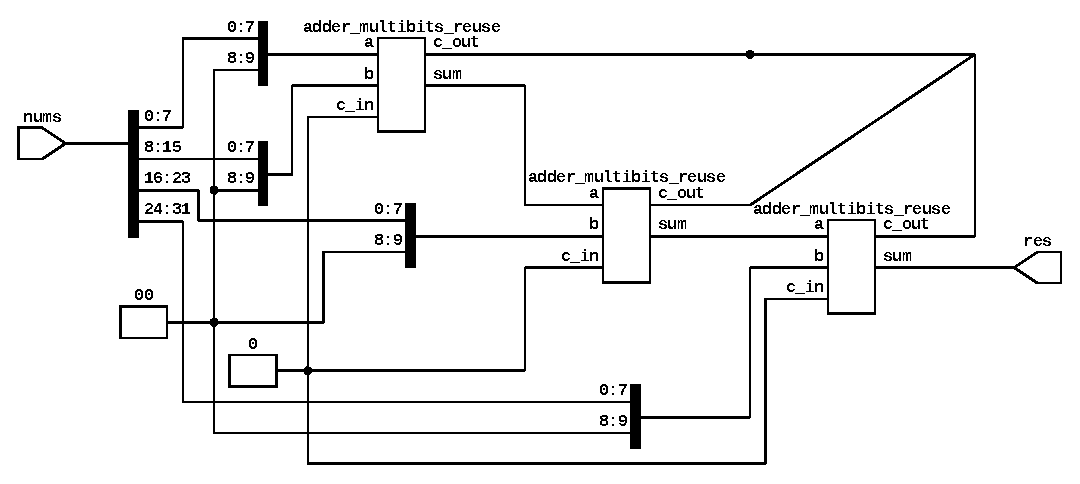
\includegraphics{images/adder_k_numbers.pdf}
	    \caption{Сумматор для четырёх 8-битных чисел}
	    \label{fig:adder_k_numbers}
        \end{figure}

	На вход модуля подаётся массив из чисел, которые необходимо сложить. Вначале вычисляется максимальная разрядность результата суммы, которая в данном случае равна 10 битам. Следовательно, все модули \verb|adder_multibits_reuse| параметризуются этой разрядностью и все 8-битные числа, которые подаются на входы $a$ и $b$ этих модулей, дополняются слева двумя нулевыми битами, так как модуль \verb|adder_multibits_reuse| работает с числами одинаковой разрядности. Также, так как известна итоговая максимальная разрядность, то переполнения при сложении двух чисел не будет. Поэтому входы $c\_in$, отвечающие за входной бит переполнения, и выходы $c\_out$, отвечающие за выходной бит переполнения, модулей \verb|adder_multibits_reuse| не используются. Поэтому на все $c\_in$ подаётся бит $0$, а провода из $c\_out$ ни к чему не подсоединены.

    \item В пятом задании нужно было реализовать сумматор k чисел типа int. Это задание было выполнено аналогично четвёртому: с помощью каскадного подключения модулей, складывающих два числа типа int. Модуль, складывающий два числа типа int, был написан дополнительно.

    \item Шестое задание требовало создать модуль для свёртки битвектора фиксированного, но параметризуемого размера для любой логической операции. Модуль был реализован для логического ИЛИ с помощью каскадного подключения вентилей ИЛИ. В качестве логической операции операция ИЛИ была выбрана случайно, так как реализация модулей для других логических операций отличалась бы незначительно.

    \item Седьмое задание заключалось в реализации модуля из шестого задания, но для одной из операций, реализованных в заданиях 1 и 2. В решении использовалось каскадное подключение модулей, реализующих дизъюнкцию. Таким образом, написанный в седьмом задании модуль для свёртки битвектора может в качесте модуля дизъюнкции использовать любой модуль с подходящей реализацией и названием, в том числе и модули дизъюнкции написанные в первом и втором заданиях.
\end{itemize}

\subsection{Блок 4:}

\begin{itemize}
	\item Первое задание в данном блоке требовало реализовать мультиплексор 4:1 через логические операторы И, ИЛИ, НЕ. Сначала в качестве решения был написан модуль, который от каждого входного бита в зависимости от значения селектора берёт либо 0, либо значение этого бита, а в конце все полученные биты скрещивает оператором ИЛИ.

		Например, пусть селектор равен $\overline{ab}$, где $a, b$~--- биты, а первый входной бит равен $in_0$. Тогда, скрестив $in_0$ оператором И с НЕ($a$ ИЛИ $b$), мы получим $in_0$ тогда и только тогда, когда $a = 0$ и $b = 0$, то есть селектор равен $00$, а в остальных случаях получится $0$. Тогда, если второй, третий и четвёртый входной биты равны соответственно $in_1, in_2$ и $in_3$, итоговой формулой для результата будет:
		$$
		(in_0 \land \lnot(a \lor b)) \lor (in_1 \land \lnot(a) \land b) \lor (in_2 \land a \land \lnot(b)) \lor (in_3 \land a \land b)
		$$
	В этой формуле три скобки всегда будут нулевые, а оставшаяся будет содержать значение выбранного селектором бита.

	Сгенерированная логическая схема модуля представлена на рисунке~\ref{fig:mux_4to1_logic}.
	\begin{figure}[H]
	    \centering
            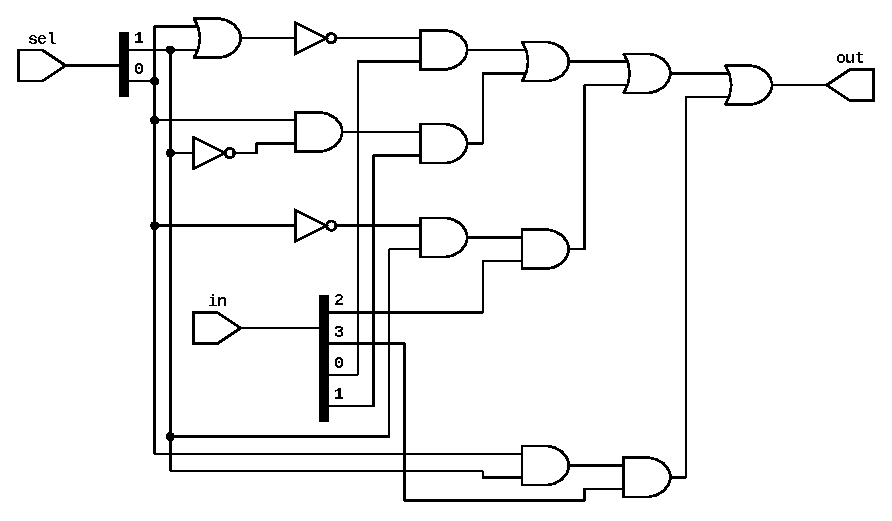
\includegraphics{images/mux_4to1_logic.pdf}
	    \caption{Мультиплексор 4:1~--- первый вариант схемы}
	    \label{fig:mux_4to1_logic}
	\end{figure}

		Как видно, данная реализация модуля требует 14 логических вентилей, что довольно избыточно. Поэтому был реализован ещё один мультиплексор 4:1, который сначала параллельно выбирает один бит из двух младших входных бит и один бит из двух старших входных бит, а потом из них выбирает результирующий бит. Алгоритм выбора такой: если младший бит селектора равен 0, то результирующим битом будет либо первый входной бит, либо третий, поэтому из двух младших входных бит и двух старших входных бит выбираем соответственно первый и третий входные биты. Если же младший бит селектора равен 1, то берём второй и четвёртый биты. После, если старший бит селектора равен 0, то на выходе должен быть либо первый, либо второй входной бит, поэтому выбираем бит, выбранный ранее из двух младших входных бит. Если же старший бит селектора равен 1, то выбираем бит, выбранный ранее из двух старших входных бит. Такой модуль уже требует 11 логических вентилей вместо 14 и имеет логическую схему, представленную на рисунке~\ref{fig:mux_4to1_logic_optimized}.
	\begin{figure}[H]
	    \centering
            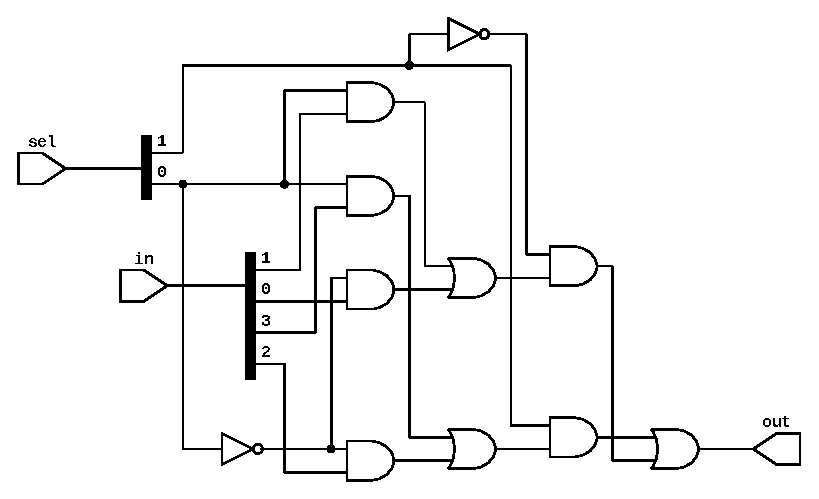
\includegraphics{images/mux_4to1_logic_optimized.pdf}
	    \caption{Оптимизированная версия мультиплексора 4:1}
	    \label{fig:mux_4to1_logic_optimized}
        \end{figure}

        Также для мультиплексора 4:1 был написан тест.

    \item Во втором задании было необходимо реализовать импликацию через мультиплексор 2:1. Решение использует один данный мультиплексор, который при входных битах a и b выбирает b при a = 1, иначе 1.

    \item Третье задание требовало реализации Look-Up Table для стрелки Пирса. В решении использовался один мультиплексор 4:1, который в качестве селектора принимает сконкатенированные входные биты, а в качестве последовательности битов для выбора всегда принимает 0001 (последний бит~--- самый младший). Тогда этот мультиплексор будет возвращать 1 тогда и только тогда, когда оба входных бита нулевые, поэтому он служит таблицей истинности для стрелки Пирса. Логическая схема модуля представлена на рисунке~\ref{fig:lut_peirce_arrow}.
	\begin{figure}[H]
	    \centering
            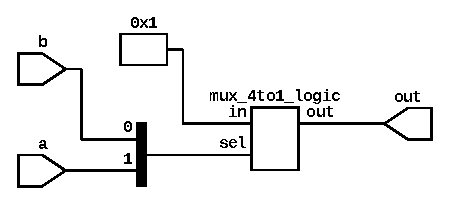
\includegraphics{images/lut_peirce_arrow.pdf}
	    \caption{Look-Up Table для стрелки Пирса}
	    \label{fig:lut_peirce_arrow}
	\end{figure}

\item В четвёртом задании было необходимо написать модуль, использующий только мультиплексоры 2:1, который принимает биты a, b, c и возвращает результат трёхместного отношения \lnot(a \lor\ b) \land\ c. Для того чтобы для решения задачи было достаточно двух мультиплексоров 2:1, исходное отношение было преобразовано в \lnot b \land\ (\lnot a \land\ c). Теперь достаточно посчитать два выражения вида \lnot x \land\ y, которые можно вычислить одним мультиплексором 2:1 так: если x = 0, то выбираем y, иначе 0. Таким образом, имеем схему модуля, представленную на рисунке~\ref{fig:solution}.
	\begin{figure}[H]
	    \centering
            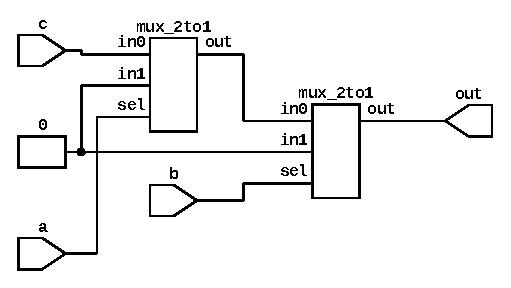
\includegraphics{images/solution.pdf}
	    \caption{Модуль, вычисляющий \lnot(a \lor\ b) \land\ c}
	    \label{fig:solution}
        \end{figure}
\end{itemize}

При выполнении заданий для исполнения программ на языке SystemVerilog использовался симулятор Icarus Verilog. Для генерации схем из модулей использовались утилиты Yosys и netlistsvg.

\section{Тестирование}

Все написанные тесты, кроме теста для первого задания 4 блока, проверяют корректность модулей с помощью заранее известных таблиц истинности. Для каждого блока создан отдельный скрипт \verb|build_and_test_all.sh|, при запуске которого исполняются тесты для всех заданий данного блока, для которых эти тесты есть. Также для тестов настроено CI на github.

\section{Заключение}

В ходе выполнения работы получены следующие результаты.

\begin{itemize}
	\item Решены все задачи из второго блока курса, что позволило научиться написанию простейших модулей и тестов к ним на языке SystemVerilog.
    \item Решены все задачи из третьего блока курса, благодаря чему получен навык написания немного более сложных модулей.
    \item Решены все задачи из четвёртого блока курса, что позволило обучиться работе с мультиплексорами.
    \item Кроме того, в процессе выполнения работы в курсе было обнаружено несколько опечаток, которые были исправлены\footnote{Ссылки на принятые в репозиторий курса запросы на изменения, содержащие исправления опечаток: \url{https://github.com/Lamagraph/intro-to-fpga-with-clash/pull/66} (дата обращения: 08.05.2026); \url{https://github.com/Lamagraph/intro-to-fpga-with-clash/pull/72} (дата обращения: 08.05.2026)}.
\end{itemize}

Таким образом, были получены базовые навыки разработки на языке SystemVerilog, что и являлось целью учебной практики.

Репозиторий с решениями задач: \url{https://github.com/meow79/FPGA\_learning}

\end{document}
